\section{Relational algebra in \dbsp}\label{sec:relational}

Results in \secref{sec:streams} apply to streams of arbitrary group
values.  In this section we turn our attention to using these results
in the context of relational databases.

However, we face a technical problem: the $\I$ and $\D$ operators were
defined on abelian groups, and relational databases in general are
not abelian groups, since they operate on sets.  Fortunately,
there is a well-known tool in the database literature
which converts set operations into group operations by using \zrs
(also called z-relations~\cite{green-pods07}) instead of sets.

We start by defining the \zrs group, and then we explain how
relational queries are converted into \dbsp circuits over \zrs.

\subsection{\zrs as an abelian group}

Given a set $A$ we define \defined{\zrs}\footnote{Also called $\Z$-relations elsewhere~\cite{green-tcs11}.}
over $A$ as functions with \emph{finite support} from $A$ to $\Z$ (i.e., which are 0 almost everywhere).
These are functions $f: A \rightarrow \Z$ where
$f(x) \not= 0$ for at most a finite number of values $x \in A$.
We also write $\Z[A]$ for the type of \zrs with elements from $A$.
The values in $\Z[A]$ can also be thought as being key-value maps with
keys in $A$ and values in $\Z$, justifying the array indexing notation.

Since $\Z$ is an abelian group, $\Z[A]$ is also an abelian group.  This group
$(\Z[A], +_{\Z[A]}, 0_{\Z[A]}, -_{\Z{A}})$ has addition and subtraction defined pointwise:
$$(f +_{\Z[A]} g)(x) = f(x) + g(x) . \forall x \in A.$$
The $0$ element of $\Z[A]$ is the function $0_{\Z[A]}$ defined by $0_{\Z[A]}(x) = 0 . \forall x \in A$.
(In fact, since $\Z$ is a ring, $\Z[A]$ is also ring, endowed with a multiplication operation,
also defined pointwise.)

A particular \zr $m \in \Z[A]$ can be denoted by enumerating the inputs that map to non-zero values and
their multiplicities:
$m = \{ x_1 \mapsto w_1, \dots, x_n \mapsto w_n \}$.
We call $w_i \in Z$ the \defined{multiplicity} (or weight)
of $x_i \in A$.  Multiplicities can be negative.
We write that $x \in m$ for $x \in A$, iff $m[x] \not= 0$.

For example, let's consider a concrete \zr $R \in \Z[\texttt{string}]$,
defined by $R = \{ \texttt{joe} \mapsto 1, \texttt{anne} \mapsto -1 \}$.
$R$ has two elements in its domain,
\texttt{joe} with a multiplicity of 1 (so $R[\texttt{joe}] = 1$),
and \texttt{anne} with a multiplicity of $-1$.
We say \texttt{joe} $\in R$ and \texttt{anne} $\in R$.

Given a \zr $m \in \Z[A]$ and a value $v \in A$, we overload the array index notation
$m[v]$ to denote the multiplicity of the element $v$ in $m$.
Thus we write $R[\texttt{anne}] = -1$.
When $c \in \Z$, and $v \in A$ we also write $c \cdot v$ for the \defined{singleton} \zr $\{
v \mapsto c \}$.  In other words, $3 \cdot \texttt{frank} = \{ \texttt{frank} \mapsto 3 \}$.
We extend scalar multiplication to operate on \zrs: for $c \in Z, m \in \Z[A]$,
$c \cdot m \defn \sum_{x \in m} (c \cdot m[x]) \cdot x$.  We then have
$2 \cdot R = \{ \texttt{joe} \mapsto 2, \texttt{anne} \mapsto -2 \}$: multiplying
each row weight by 2.

We define the \defined{size} of a \zr as the size of its support set, and we use the
modulus symbol to represent the size: $|m| \defn \sum_{x \in m} 1$.  So $|R| = 2$.

\subsection{Sets, bags, and \zrs}

\zrs generalize sets and bags.
Given a set with elements from $A$, it can be represented as a \zr $\Z[A]$
by associating a weight of 1 with each set element.  The function $\mbox{tozset}: 2^A \to \Z[A]$,
defined as $\mbox{tozset}(s) = \sum_{x \in s} 1 \cdot x$,
converts a set to a \zr by associating a multiplicity of 1 with each set element.
Thus $\mbox{tozset}(\{ \code{joe}, \code{anne} \}) = \{ \code{joe} \mapsto 1, \code{anne} \mapsto 1 \}$.

\begin{definition}
We say that a \zr represents a \defined{set} if the multiplicity of every
element is one.  We define a function to check this property
$\isset : \Z[A] \rightarrow \B$\index{isset}, given by:
$$\isset(m) \defn \left\{
\begin{array}{ll}
  \mbox{true} & \mbox{ if } m[x] = 1, \forall x \in m \\
  \mbox{false} & \mbox{ otherwise}
\end{array}
\right.
$$
\end{definition}
For our example $\isset(R) = \mbox{false}$, since $R[\texttt{anne}] = -1$.
$\isset(\mbox{tozset}(m)) = \mbox{true}$ for any set $m \in 2^A$.

\begin{definition}
We say that a \zr is \defined{positive} (or a \defined{bag}) if the multiplicity of every element is
positive. We define a function to check this property
$\ispositive : \Z[A] \rightarrow \B$\index{ispositive}, given by
$$\ispositive(m) \defn \left\{
\begin{array}{ll}
  \mbox{true} & \mbox{ if } m[x] \geq 0, \forall x \in A \\
  \mbox{false} & \mbox{ otherwise}
\end{array}
\right.$$
\end{definition}
For our example $\ispositive(R) = \mbox{false}$, since $R[\texttt{anne}] = -1$,
but $\isset(m) \Rightarrow \ispositive(m). \forall m \in \Z[A]$.

We also write $m \geq 0$ when $m$ is
positive.  For positive $m, n$ we write $m \geq n$ for $m, n
\in \Z[A]$ iff $m - n \geq 0$.  The relation $\geq$ is a partial order.

\begin{definition}
The function $\distinct: \Z[A] \rightarrow \Z[A]$\index{distinct}
projects a \zr into an underlying set (but \emph{the result is
  still a \zr}).  The definition is $\forall x \in A$
$$\distinct(m)[x] \defn \left\{
\begin{array}{ll}
  1 & \mbox{ if } m[x] > 0 \\
  0 & \mbox{ otherwise}
\end{array}
\right.
$$
\end{definition}
$\distinct(R) = \{ \texttt{joe} \mapsto 1 \}$.

$\distinct$ ``removes'' elements with negative multiplicities.  $\zpp{\distinct}$.

Circuits derived from relational program will only operate with positive \zrs;
non-positive values will be only used to represent \emph{changes} to \zrs
(a change with negative weights will remove elements from a \zr).

\begin{proposition}
$\distinct$ is idempotent: $\distinct = \distinct \circ \distinct$.
\end{proposition}

\begin{proposition}
For any $m \in \Z[A]$ we have: $\isset(\distinct(m))$ and \\
$\ispositive(\distinct(m))$.
\end{proposition}

We call a function $f : \Z[I] \rightarrow \Z[O]$ \defined{positive} if
$\forall x \in \Z[I], x \geq 0_{\Z[I]} \Rightarrow f(x) \geq 0_{\Z[0]}$.
We extend the notation used for \zrs for functions as well: $\ispositive(f)$.

\paragraph{Correctness of the \dbsp implementations}

The function $\mbox{toset}: \Z[A] \to 2^A$, defined as $\mbox{toset}(m) =
\cup_{x \in \distinct(m)} \{ x \}$, converts a \zr into a set.

A relational query $f$ that transforms
a set $V$ into a set $U$ will be implemented by a \dbsp computation $f'$ on
\zrs.  The correctness of the implementation requires that the following
diagram commutes:

\begin{center}
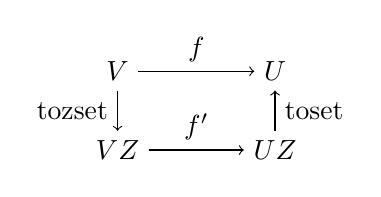
\begin{tikzpicture}
  \node[] (V) {$V$};
  \node[below of=V] (VZ) {$VZ$};
  \node[right of=V, node distance=2cm] (U) {$U$};
  \node[below of=U] (UZ) {$UZ$};
  \draw[->] (V) -- node (f) [above] {$f$} (U);
  \draw[->] (V) --  node (s) [left] {tozset}(VZ);
  \draw[->] (VZ) -- node (f) [above] {$f'$} (UZ);
  \draw[->] (UZ) -- node (d) [right] {toset} (U);
\end{tikzpicture}
\end{center}

\textbf{Remark:} We can generalize the notion of \zrs to functions $m: A \to \mathbf{G}$ for a
ring $\mathbf{G}$ other than $\Z$.  The properties we need from the ring structure are the
following: the ring must be a commutative group (needed for defining $\I$, $\D$, and $\zm$),
the multiplication operation must distribute over addition (needed to define
Cartesian products), and there must be a notion of positive values, needed
to define the $\distinct$ function.  Rings such as $\mathbb{Q}$ or $\mathbb{R}$
would work perfectly.

\subsection{Streams over \zrs}

Since all the results from Section~\ref{sec:streams} are true for streams
over an arbitrary abelian group, they extend to streams where the elements
are \zrs.  In the rest of this text we only consider streams of the form $\stream{\Z[A]}$, for
some element type $A$.

An example of a stream of \zrs is \\ $s = \sv{0 R -1\cdot{R} 2\cdot{R} -2\cdot{R}}$.
We have $s[2] = -R = \{ \texttt{joe} \mapsto -1, \texttt{anne} \mapsto 1 \}$.

\begin{definition}
A stream $s \in \stream{\Z[A]}$ is \defined{positive} if every value of the stream is positive:
$s[t] \geq 0 . \forall t \in \N$.
\end{definition}



\begin{definition}
A stream $s \in \stream{\Z[A]}$ is \defined{monotone} if $s[t] \geq s[t-1], \forall t \in \N$.
\end{definition}

\begin{lemma}
Given a positive stream $s \in \stream{\Z[A]}$ the stream $\I(s)$ is monotone.
\end{lemma}
\begin{proof}
  Let us compute $\I(s)[t + 1] - \I(s)[t] = \sum_{i \leq t+1}s[i] -
  \sum_{i \leq t}s[i] = s[t+1] \geq 0$, by commutativity and positivity of $s$.
\end{proof}

\begin{lemma}
Given a monotone stream $s \in \stream{\Z[A]}$, the
elements of the stream $\D(s)$ are positive.
\end{lemma}
\begin{proof}
  By the definition of monotonicity $s[t+1] \geq s[t]$.  By definition
  of $\D$ we have $\D(s)[t+1] = s[t+1] - s[t] \geq 0$.
\end{proof}

\subsection{Implementing the relational algebra}\label{sec:relational-operators}

The fact that the relational algebra can be implemented by computations
on \zrs has been shown before, e.g.~\cite{green-pods07}.  The translation
of the core relational operators is summarized in Table~\ref{tab:relational} and discussed below.

\begin{table*}
\begin{center}
\footnotesize
\begin{tabular}{|m{1.2cm}m{4.2cm}m{5cm}|} \hline
Operation & SQL example & \dbsp circuit  \\ \hline
Composition &
 \begin{lstlisting}[language=SQL]
SELECT DISTINCT ... FROM
(SELECT ... FROM ...)
\end{lstlisting}
 &
 \begin{tikzpicture}[auto,>=latex]
  \node[] (I) {\code{I}};
  \node[block, right of=I] (CI) {$C_I$};
  \draw[->] (I) -- (CI);
  \node[block, right of=CI] (CO) {$C_O$};
  \node[right of=CO] (O) {\code{O}};
  \draw[->] (CI) -- (CO);
  \draw[->] (CO) -- (O);
\end{tikzpicture}
\\ \hline
Union &
\begin{lstlisting}[language=SQL]
(SELECT * FROM I1)
UNION
(SELECT * FROM I2)
\end{lstlisting}
&
\begin{tikzpicture}[auto,>=latex]
  \node[] (input1) {\code{I1}};
  \node[below of=input1, node distance=.4cm] (midway) {};
  \node[below of=midway, node distance=.4cm] (input2) {\code{I2}};
  \node[block, shape=circle, right of=midway, inner sep=0in] (plus) {$+$};
  \node[block, right of=plus, node distance=1.5cm] (distinct) {$\distinct$};
  \node[right of=distinct, node distance=1.5cm] (output) {\code{O}};
  \draw[->] (input1) -| (plus);
  \draw[->] (input2) -| (plus);
  \draw[->] (plus) -- (distinct);
  \draw[->] (distinct) -- (output);
\end{tikzpicture}
\\ \hline
Projection &
\begin{lstlisting}[language=SQL]
SELECT DISTINCT I.c
FROM I
\end{lstlisting}
&
\begin{tikzpicture}[auto,>=latex]
  \node[] (input) {\code{I}};
  \node[block, right of=input] (pi) {$\pi$};
  \node[block, right of=pi, node distance=1.5cm] (distinct) {$\distinct$};
  \node[right of=distinct, node distance=1.5cm] (output) {\code{O}};
  \draw[->] (input) -- (pi);
  \draw[->] (pi) -- (distinct);
  \draw[->] (distinct) -- (output);
\end{tikzpicture}
\\ \hline
Filtering &
\begin{lstlisting}[language=SQL]
SELECT * FROM I
WHERE p(I.c)
\end{lstlisting}
&
\begin{tikzpicture}[auto,>=latex]
  \node[] (input) {\code{I}};
  \node[block, right of=input] (map) {$\sigma_P$};
  \node[block, right of=map, node distance=1.4cm] (distinct) {$\distinct$};
  \node[right of=distinct] (output) {\code{O}};
  \draw[->] (input) -- (map);
  \draw[->] (map) -- (distinct);
  \draw[->] (distinct) -- (output);
\end{tikzpicture}
\\ \hline
Selection &
\begin{lstlisting}[language=SQL]
SELECT DISTINCT f(I.c, ...)
FROM I
\end{lstlisting}
&
\begin{tikzpicture}[auto,>=latex]
  \node[] (input) {\code{I}};
  \node[block, right of=input, node distance=1.5cm] (map) {$\mbox{map}(f)$};
  \node[block, right of=map, node distance=1.5cm] (distinct) {$\distinct$};
  \node[right of=distinct, node distance=1.5cm] (output) {\code{O}};
  \draw[->] (input) -- (map);
  \draw[->] (map) -- (distinct);
  \draw[->] (distinct) -- (output);
\end{tikzpicture}
\\ \hline
\parbox[b][][t]{1cm}{
Cartesian \\
product} &
\begin{lstlisting}[language=SQL]
SELECT I1.*, I2.*
FROM I1, I2
\end{lstlisting}
&
\begin{tikzpicture}[auto,>=latex]
  \node[] (i1) {\code{I1}};
  \node[below of=i1, node distance=.4cm] (midway) {};
  \node[below of=midway, node distance=.4cm] (i2) {\code{I2}};
  \node[block, right of=midway] (prod) {$\times$};
  \node[right of=prod] (output) {\code{O}};
  \draw[->] (i1) -| (prod);
  \draw[->] (i2) -| (prod);
  \draw[->] (prod) -- (output);
\end{tikzpicture}
\\ \hline
Join &
\begin{lstlisting}[language=SQL]
SELECT I1.*, I2.*
FROM I1 JOIN I2
ON I1.c1 = I2.c2
\end{lstlisting}
&
\begin{tikzpicture}[auto,>=latex]
  \node[] (i1) {\code{I1}};
  \node[below of=i1, node distance=.4cm] (midway) {};
  \node[below of=midway, node distance=.4cm] (i2) {\code{I2}};
  \node[block, right of=midway] (prod) {$\bowtie$};
  \node[right of=prod] (output) {\code{O}};
  \draw[->] (i1) -| (prod);
  \draw[->] (i2) -| (prod);
  \draw[->] (prod) -- (output);
\end{tikzpicture}
\\ \hline
Intersection &
\begin{lstlisting}[language=SQL]
(SELECT * FROM I1)
INTERSECT
(SELECT * FROM I2)
\end{lstlisting}
&
\begin{tikzpicture}[auto,>=latex]
  \node[] (i1) {\code{I1}};
  \node[below of=i1, node distance=.4cm] (midway) {};
  \node[below of=midway, node distance=.4cm] (i2) {\code{I2}};
  \node[block, right of=midway] (prod) {$\bowtie$};
  \node[right of=prod] (output) {\code{O}};
  \draw[->] (i1) -| (prod);
  \draw[->] (i2) -| (prod);
  \draw[->] (prod) -- (output);
\end{tikzpicture}
\\ \hline
Difference &
\begin{lstlisting}[language=SQL]
SELECT * FROM I1
EXCEPT
SELECT * FROM I2
\end{lstlisting}
&
\begin{tikzpicture}[auto,>=latex, node distance=.7cm]
  \node[] (i1) {\code{I1}};
  \node[below of=i1, node distance=.4cm] (midway) {};
  \node[below of=midway, node distance=.4cm] (i2) {\code{I2}};
  \node[block, shape=circle, inner sep=0in, right of=i2] (m) {$-$};
  \node[block, right of=midway, shape=circle, inner sep=0in, node distance=1.3cm] (plus) {$+$};
  \node[block, right of=plus, node distance=1.5cm] (distinct) {$\distinct$};
  \node[right of=distinct, node distance=1.5cm] (output) {\code{O}};
  \draw[->] (i1) -| (plus);
  \draw[->] (i2) -- (m);
  \draw[->] (m) -| (plus);
  \draw[->] (plus) -- (distinct);
  \draw[->] (distinct) -- (output);
\end{tikzpicture}
\\ \hline
\end{tabular}
\caption{Implementation of SQL relational set operators in \dbsp.
Each query assumes that inputs \code{I}, \code{I1}, \code{I2}, are sets and it
produces output sets.\label{tab:relational}}
\end{center}
\end{table*}

The translation is fairly straightforward, but many operators require
the application of a $\distinct$ to produce sets.  The correctness of
this implementation is predicated on the global circuit inputs being
sets as well.

\subsubsection{Query composition}

A composite query is translated by compiling each sub-query separately into a circuit
and composing the respective circuits.

For example, consider the following SQL query:

\begin{lstlisting}[language=SQL]
SELECT ... FROM (SELECT ... FROM ...)
\end{lstlisting}

\noindent given circuits $C_O$ implementing the outer query and $C_I$
implementing the inner query, the translation of the composite query is:

\begin{center}
\begin{tikzpicture}[auto,>=latex]
  \node[] (I) {\code{I}};
  \node[block, right of=I] (CI) {$C_I$};
  \draw[->] (I) -- (CI);
  \node[block, right of=CI] (CO) {$C_O$};
  \node[right of=CO] (O) {\code{O}};
  \draw[->] (CI) -- (CO);
  \draw[->] (CO) -- (O);
\end{tikzpicture}
\end{center}

We have $\ispositive(C_I) \land \ispositive(C_0) \Rightarrow \ispositive(C_O \circ C_I)$
and $\zpp{C_I} \land \zpp{C_O} \Rightarrow \zpp{C_O \circ C_I}$.

\subsubsection{Set union}

Consider the following SQL query:

\begin{lstlisting}[language=SQL]
(SELECT * FROM I1) UNION (SELECT * FROM I2)
\end{lstlisting}

The following circuit implements the union program:

\begin{center}
\begin{tikzpicture}[auto,>=latex]
  \node[] (input1) {\code{I1}};
  \node[below of=input1, node distance=.4cm] (midway) {};
  \node[below of=midway, node distance=.4cm] (input2) {\code{I2}};
  \node[block, shape=circle, right of=midway, inner sep=0in] (plus) {$+$};
  \node[block, right of=plus, node distance=1.5cm] (distinct) {$\distinct$};
  \node[right of=distinct, node distance=1.5cm] (output) {\code{O}};
  \draw[->] (input1) -| (plus);
  \draw[->] (input2) -| (plus);
  \draw[->] (plus) -- (distinct);
  \draw[->] (distinct) -- (output);
\end{tikzpicture}
\end{center}

Given \zrs $a, b \in \Z[I]$ s.t. $\isset(a)$ and $\isset(b)$, their \emph{set union}
can be computed as: $\cup: \Z[I] \times \Z[I] \rightarrow \Z[I]$,  $$a
\cup b \defn \distinct(a +_{\Z[I]} b).$$
The $\distinct$ application is necessary to provide the set semantics.

\subsubsection{Projection}
Consider a query such as:

\begin{lstlisting}[language=SQL]
SELECT I.c FROM I
\end{lstlisting}

We can assume without loss of generality that table \code{I} has two columns, and that
a single column is preserved in the projection.
Hence the type of \code{I} is $\Z[A_0 \times A_1]$ while the result has type is $\Z[A_0]$.
In terms of \zrs, the projection of a \zr $i$ on $A_0$ is defined as: $$\pi(i)[y] =
\sum_{x \in i, x|_0 = y} i[x]$$
\noindent where $x|_0$ is first component of the tuple $x$.
In other words, the multiplicity of a tuple in the result is the sum
of the multiplicities of all input tuples that project to it.

The circuit for a projection query is:

\begin{center}
\begin{tikzpicture}[auto,>=latex]
  \node[] (input) {\code{I}};
  \node[block, right of=input] (pi) {$\pi$};
  \node[block, right of=pi, node distance=1.5cm] (distinct) {$\distinct$};
  \node[right of=distinct, node distance=1.5cm] (output) {\code{O}};
  \draw[->] (input) -- (pi);
  \draw[->] (pi) -- (distinct);
  \draw[->] (distinct) -- (output);
\end{tikzpicture}
\end{center}

The $\distinct$ is necessary to convert the result to a set.\\
$\pi$ is linear; $\ispositive(\pi), \zpp{\pi}$.

\subsubsection{Selection}

We generalize the SQL selection operator to allow it to apply an arbitrary function to each row of the
selected set.
Given a function $f : A \rightarrow B$, the mathematical \defined{map} operator ``lifts'' the
function $f$ to operate on \zrs: $\map(f) : \Z[A] \rightarrow \Z[B]$.  A map operator
appears in SQL due to the use of expressions in the SELECT clause, as in the following example:

\begin{lstlisting}[language=SQL]
SELECT f(I.c) FROM I
\end{lstlisting}

The circuit implementation of this query is:

\begin{center}
\begin{tikzpicture}[auto,>=latex]
  \node[] (input) {\code{I}};
  \node[block, right of=input, node distance=1.5cm] (map) {$\mbox{map}(f)$};
  \node[block, right of=map, node distance=2cm] (distinct) {$\distinct$};
  \node[right of=distinct, node distance=1.5cm] (output) {\code{O}};
  \draw[->] (input) -- (map);
  \draw[->] (map) -- (distinct);
  \draw[->] (distinct) -- (output);
\end{tikzpicture}
\end{center}

For any function $f$ we have the following properties:
$\map(f)$ is linear, $\ispositive(\map(f)), and \zpp{\map(f)}.$

\subsubsection{Filtering}

Filtering occurs in SQL through a WHERE clause, as in the following example:

\noindent
\begin{lstlisting}[language=SQL]
SELECT * FROM I WHERE p(I.c)
\end{lstlisting}

Let us assume that we are filtering with a predicate
$P: A \rightarrow \B$.  We define the following function $\sigma_P: \Z[A] \rightarrow \Z[A]$ as:
$$\sigma_P(m)[t] = \left\{
\begin{array}{ll}
  m[t] \cdot t & \mbox{ if } P(t) \\
  0 & \mbox{ otherwise } \\
\end{array}
\right.
$$

The circuit for filtering with a predicate $P$ is:

\begin{center}
\begin{tikzpicture}[auto,>=latex]
  \node[] (input) {\code{I}};
  \node[block, right of=input] (map) {$\sigma_P$};
  \node[right of=map] (output) {\code{O}};
  \draw[->] (input) -- (map);
  \draw[->] (map) -- (output);
\end{tikzpicture}
\end{center}

For any predicate $P$ we have $\isset(i) \Rightarrow
\isset(\sigma_P(i))$ and $\ispositive(\sigma_P)$.  Thus a $\distinct$
is not needed.  $\sigma_P$ is linear and $\zpp{\sigma_P}$.

\subsubsection{Cartesian products}

Consider this SQL query performing a Cartesian product
between sets \code{I1} and \code{I2}:

\begin{lstlisting}[language=SQL]
SELECT I1.*, I2.* FROM I1, I2
\end{lstlisting}

We first define a product operation on \zrs.
For $a \in \Z[A]$ and $b \in \Z[B]$ we define $a \times b \in \Z[A \times B]$ by
$$(a \times b)((x,y)) \defn a[x] \times b[y] . \forall x \in a, y \in b.$$
The weight of a pair in the result is the product of the weights of the
elements in the sources.  The circuit for the query is:

\begin{center}
\begin{tikzpicture}[auto,>=latex]
  \node[] (i1) {\code{I1}};
  \node[below of=i1, node distance=.5cm] (midway) {};
  \node[below of=midway, node distance=.5cm] (i2) {\code{I2}};
  \node[block, right of=midway] (prod) {$\times$};
  \node[right of=prod] (output) {\code{O}};
  \draw[->] (i1) -| (prod);
  \draw[->] (i2) -| (prod);
  \draw[->] (prod) -- (output);
\end{tikzpicture}
\end{center}

$\isset(x) \land \isset(y) \Rightarrow \isset(x \times y).$
$\times$ is bilinear, $\ispositive(\times), \zpp{\times}$.

\subsubsection{Joins}

As is well-known, joins can be modeled as Cartesian products
followed by filtering.  Since a join is a composition of a bilinear
and a linear operator, it is also a bilinear operator.
$\ispositive(\bowtie), \zpp{\bowtie}.$

In practice joins are very important computationally, and they are
implemented by a built-in scalar function on \zrs:

$$(a \bowtie b)((x,y)) \defn a[x] \times b[y] \mbox{ if } x|_{c1} = y|_{c2}.$$

\begin{center}
\begin{tikzpicture}[auto,>=latex]
  \node[] (i1) {\code{I1}};
  \node[below of=i1, node distance=.5cm] (midway) {};
  \node[below of=midway, node distance=.5cm] (i2) {\code{I2}};
  \node[block, right of=midway] (prod) {$\bowtie$};
  \node[right of=prod] (output) {\code{O}};
  \draw[->] (i1) -| (prod);
  \draw[->] (i2) -| (prod);
  \draw[->] (prod) -- (output);
\end{tikzpicture}
\end{center}

\subsubsection{Set intersection}

Set intersection is a special case of join, where both relations have the same schema.
It follows that set intersection is bilinear,
and has the zero-preservation property.

\subsubsection{Set difference}  Consider the following query:

\begin{lstlisting}[language=SQL]
SELECT * FROM I1 EXCEPT SELECT * FROM I2
\end{lstlisting}

We define the set difference on \zrs as follows:
$\setminus: \Z[I] \times \Z[I] \rightarrow \Z[I]$, where $$i_1
\setminus i_2 = \distinct(i_1 - i_2).$$  Note
that we have $\forall i_1, i_2, \ispositive(i_1 \setminus
i_2)$ due to the $\distinct$ operator.
The circuit computing the above query is:

\begin{center}
\begin{tikzpicture}[auto,>=latex, node distance=.7cm]
  \node[] (i1) {\code{I1}};
  \node[below of=i1, node distance=.4cm] (midway) {};
  \node[below of=midway, node distance=.4cm] (i2) {\code{I2}};
  \node[block, shape=circle, inner sep=0in, right of=i2] (m) {$-$};
  \node[block, right of=midway, shape=circle, inner sep=0in, node distance=1.3cm] (plus) {$+$};
  \node[block, right of=plus, node distance=1.5cm] (distinct) {$\distinct$};
  \node[right of=distinct, node distance=1.5cm] (output) {\code{O}};
  \draw[->] (i1) -| (plus);
  \draw[->] (i2) -- (m);
  \draw[->] (m) -| (plus);
  \draw[->] (plus) -- (distinct);
  \draw[->] (distinct) -- (output);
\end{tikzpicture}
\end{center}
